\section{Empirical Experiments}
\label{sec:empirical}
We evaluate the downstream task performance of LoRA on RoBERTa~\citep{liu2019roberta}, DeBERTa~\citep{he2021deberta}, and GPT-2~\citep{radford_language_nodate}, before scaling up to GPT-3 175B~\citep{brown_language_2020}.
Our experiments cover a wide range of tasks, from natural language understanding (NLU) to generation (NLG).
Specifically, we evaluate on the GLUE~\citep{wang2019glue} benchmark for RoBERTa and DeBERTa.
We follow the setup of~\citet{li_prefix-tuning_2021} on GPT-2 for a direct comparison and add WikiSQL~\citep{DBLP:journals/corr/abs-1709-00103} (NL to SQL queries) and SAMSum~\citep{DBLP:journals/corr/abs-1911-12237} (conversation summarization) for large-scale experiments on GPT-3.
See \autoref{app:datasets} for more details on the datasets we use.
We use NVIDIA Tesla V100 for all experiments.

\subsection{Baselines}
\label{sec:expt_baselines}
To compare with other baselines broadly, we replicate the setups used by prior work and reuse their reported numbers whenever possible.
This, however, means that some baselines might only appear in certain experiments.

\textbf{Fine-Tuning (FT)} is a common approach for adaptation.
During fine-tuning, the model is initialized to the pre-trained weights and biases, and all model parameters undergo gradient updates.%
A simple variant is to update only some layers while freezing others.
We include one such baseline reported in prior work~\citep{li_prefix-tuning_2021} on GPT-2, which adapts just the last two layers ($\textbf{FT}^{\textbf{Top2}}$).

\textbf{Bias-only or BitFit} is a baseline where we only train the bias vectors while freezing everything else.
Contemporarily, this baseline has also been studied by BitFit~\citep{zaken2021bitfit}.

\textbf{Prefix-embedding tuning (PreEmbed)} inserts special tokens among the input tokens.
These special tokens have trainable word embeddings and are generally not in the model's vocabulary.
Where to place such tokens can have an impact on performance.
We focus on ``prefixing'', which prepends such tokens to the prompt, and ``infixing'', which appends to the prompt; both are discussed in~\citet{li_prefix-tuning_2021}.
We use $l_{p}$ (resp. $l_{i}$) denote the number of prefix (resp. infix) tokens.
The number of trainable parameters is $|\Theta| = d_{model} \times (l_p + l_i)$.

\textbf{Prefix-layer tuning (PreLayer)} is an extension to prefix-embedding tuning.
Instead of just learning the word embeddings (or equivalently, the activations after the embedding layer) for some special tokens, we learn the activations after every Transformer layer.
The activations computed from previous layers are simply replaced by trainable ones.
The resulting number of trainable parameters is $|\Theta| = L \times d_{model} \times (l_p + l_i)$, where $L$ is the number of Transformer layers.

\textbf{Adapter tuning} as proposed in~\citet{houlsby_parameter-efficient_2019} inserts adapter layers between the self-attention module (and the MLP module) and the subsequent residual connection.
There are two fully connected layers with biases in an adapter layer with a nonlinearity in between.
We call this original design $\textbf{Adapter}^{\textbf{H}}$.
Recently, \citet{lin-etal-2020-exploring} proposed a more efficient design with the adapter layer applied only after the MLP module and after a LayerNorm.
We call it $\textbf{Adapter}^{\textbf{L}}$.
This is very similar to another deign proposed in~\citet{pfeiffer2021adapterfusion}, which we call $\textbf{Adapter}^{\textbf{P}}$.
We also include another baseline call AdapterDrop~\citep{ruckle2020adapterdrop} which drops some adapter layers for greater efficiency ($\textbf{Adapter}^{\textbf{D}}$).
We cite numbers from prior works whenever possible to maximize the number of baselines we compare with; they are in rows with an asterisk (*) in the first column.
In all cases,  we have $|\Theta| = \hat{L}_{Adpt} \times (2 \times d_{model} \times r + r + d_{model}) + 2 \times \hat{L}_{LN} \times d_{model}$ where $\hat{L}_{Adpt}$ is the number of adapter layers and $\hat{L}_{LN}$ the number of trainable LayerNorms (e.g., in $\text{Adapter}^{\text{L}}$).

\textbf{LoRA} adds trainable pairs of rank decomposition matrices in parallel to existing weight matrices.
As mentioned in~\autoref{sec:apply_lora_to_tr}, we only apply LoRA to $W_{q}$ and $W_{v}$ in most experiments for simplicity.
The number of trainable parameters is determined by the rank $r$ and the shape of the original weights: $|\Theta| = 2 \times \hat{L}_{LoRA} \times d_{model} \times r$, where $\hat{L}_{LoRA}$ is the number of weight matrices we apply LoRA to.

\subsection{RoBERTa base/large}
\label{sec:bert_expt}


\begin{table}[t!]
  \centering
  \footnotesize
  \addtolength{\tabcolsep}{-4pt}
  \begin{tabular}{l|r|ccccccccc}
  \hline
  \toprule
  Model \& Method & \# Trainable & \multicolumn{9}{c}{} \\
         & Parameters & MNLI & SST-2 & MRPC & CoLA & QNLI & QQP & RTE & STS-B & Avg. \\
  \midrule
  $\text{RoB}_\text{base}$ (FT)* & 125.0M & \textbf{87.6} & 94.8 & 90.2 & \textbf{63.6} & 92.8 & \textbf{91.9} & 78.7 & 91.2 & 86.4 \\
  $\text{RoB}_\text{base}$ (BitFit)* & 0.1M & 84.7 & 93.7 & \textbf{92.7} & 62.0 & 91.8 & 84.0 & 81.5 & 90.8 & 85.2 \\
  $\text{RoB}_\text{base}$ ($\text{Adpt}^{\text{D}}$)* & 0.3M & 87.1\textsubscript{$\pm$.0} & 94.2\textsubscript{$\pm$.1} & 88.5\textsubscript{$\pm$1.1} & 60.8\textsubscript{$\pm$.4} & 93.1\textsubscript{$\pm$.1} & 90.2\textsubscript{$\pm$.0} & 71.5\textsubscript{$\pm$2.7} & 89.7\textsubscript{$\pm$.3} & 84.4 \\
  $\text{RoB}_\text{base}$ ($\text{Adpt}^{\text{D}}$)* & 0.9M & 87.3\textsubscript{$\pm$.1} & 94.7\textsubscript{$\pm$.3} & 88.4\textsubscript{$\pm$.1} & 62.6\textsubscript{$\pm$.9} & 93.0\textsubscript{$\pm$.2} & 90.6\textsubscript{$\pm$.0} & 75.9\textsubscript{$\pm$2.2} & 90.3\textsubscript{$\pm$.1} & 85.4 \\
  $\text{RoB}_\text{base}$ (LoRA) & 0.3M & 87.5\textsubscript{$\pm$.3} & \textbf{95.1\textsubscript{$\pm$.2}} & 89.7\textsubscript{$\pm$.7} & 63.4\textsubscript{$\pm$1.2} & \textbf{93.3\textsubscript{$\pm$.3}} & 90.8\textsubscript{$\pm$.1} & \textbf{86.6\textsubscript{$\pm$.7}} & \textbf{91.5\textsubscript{$\pm$.2}} & \textbf{87.2} \\
  \midrule
  $\text{RoB}_\text{large}$ (FT)* & 355.0M & 90.2 & \textbf{96.4} & \textbf{90.9} & 68.0 & 94.7 & \textbf{92.2} & 86.6 & 92.4 & 88.9 \\
  $\text{RoB}_\text{large}$ (LoRA) & 0.8M & \textbf{90.6}\textsubscript{$\pm$.2} & 96.2\textsubscript{$\pm$.5} & \textbf{90.9}\textsubscript{$\pm$1.2} & \textbf{68.2}\textsubscript{$\pm$1.9} & \textbf{94.9}\textsubscript{$\pm$.3} & 91.6\textsubscript{$\pm$.1} & \textbf{87.4}\textsubscript{$\pm$2.5} & \textbf{92.6}\textsubscript{$\pm$.2} & \textbf{89.0} \\
  \midrule
  $\text{RoB}_\text{large}$ ($\text{Adpt}^{\text{P}}$)$\dagger$ & 3.0M & 90.2\textsubscript{$\pm$.3} & 96.1\textsubscript{$\pm$.3} & 90.2\textsubscript{$\pm$.7} & \textbf{68.3}\textsubscript{$\pm$1.0} & \textbf{94.8}\textsubscript{$\pm$.2} & \textbf{91.9}\textsubscript{$\pm$.1} & 83.8\textsubscript{$\pm$2.9} & 92.1\textsubscript{$\pm$.7} & 88.4 \\
  $\text{RoB}_\text{large}$ ($\text{Adpt}^{\text{P}}$)$\dagger$ & 0.8M & \textbf{90.5}\textsubscript{$\pm$.3} & \textbf{96.6}\textsubscript{$\pm$.2} & 89.7\textsubscript{$\pm$1.2} & 67.8\textsubscript{$\pm$2.5} & \textbf{94.8}\textsubscript{$\pm$.3} & 91.7\textsubscript{$\pm$.2} & 80.1\textsubscript{$\pm$2.9} & 91.9\textsubscript{$\pm$.4} & 87.9 \\
  $\text{RoB}_\text{large}$ ($\text{Adpt}^{\text{H}}$)$\dagger$ & 6.0M & 89.9\textsubscript{$\pm$.5} & 96.2\textsubscript{$\pm$.3} & 88.7\textsubscript{$\pm$2.9} & 66.5\textsubscript{$\pm$4.4} & 94.7\textsubscript{$\pm$.2} & 92.1\textsubscript{$\pm$.1} & 83.4\textsubscript{$\pm$1.1} & 91.0\textsubscript{$\pm$1.7} & 87.8 \\
  $\text{RoB}_\text{large}$ ($\text{Adpt}^{\text{H}}$)$\dagger$ & 0.8M & 90.3\textsubscript{$\pm$.3} & 96.3\textsubscript{$\pm$.5} & 87.7\textsubscript{$\pm$1.7} & 66.3\textsubscript{$\pm$2.0} & 94.7\textsubscript{$\pm$.2} & 91.5\textsubscript{$\pm$.1} & 72.9\textsubscript{$\pm$2.9} & 91.5\textsubscript{$\pm$.5} & 86.4 \\
  $\text{RoB}_\text{large}$ (LoRA)$\dagger$ & 0.8M & \textbf{90.6}\textsubscript{$\pm$.2} & 96.2\textsubscript{$\pm$.5} & \textbf{90.2}\textsubscript{$\pm$1.0} & 68.2\textsubscript{$\pm$1.9} & \textbf{94.8}\textsubscript{$\pm$.3} & 91.6\textsubscript{$\pm$.2} & \textbf{85.2}\textsubscript{$\pm$1.1} & \textbf{92.3}\textsubscript{$\pm$.5} & \textbf{88.6} \\
  \midrule
  $\text{DeB}_\text{XXL}$ (FT)* & 1500.0M & 91.8 & \textbf{97.2} & 92.0 & 72.0 & \textbf{96.0} & 92.7 & 93.9 & 92.9 & 91.1 \\
  $\text{DeB}_\text{XXL}$ (LoRA) & 4.7M & \textbf{91.9}\textsubscript{$\pm$.2} & 96.9\textsubscript{$\pm$.2} & \textbf{92.6}\textsubscript{$\pm$.6} & \textbf{72.4}\textsubscript{$\pm$1.1} & \textbf{96.0}\textsubscript{$\pm$.1} & \textbf{92.9}\textsubscript{$\pm$.1} & \textbf{94.9}\textsubscript{$\pm$.4} & \textbf{93.0}\textsubscript{$\pm$.2} & \textbf{91.3} \\
  \bottomrule
  \end{tabular}
  \caption{$\text{RoBERTa}_{\text{base}}$, $\text{RoBERTa}_{\text{large}}$, and $\text{DeBERTa}_{\text{XXL}}$ with different adaptation methods on the GLUE benchmark. We report the overall (matched and mismatched) accuracy for MNLI, Matthew's correlation for CoLA, Pearson correlation for STS-B, and accuracy for other tasks. Higher is better for all metrics. * indicates numbers published in prior works. $\dagger$ indicates runs configured in a setup similar to~\cite{houlsby_parameter-efficient_2019} for a fair comparison.
  }
  \label{tab:NLU_results}
\end{table}
RoBERTa~\citep{liu2019roberta} optimized the pre-training recipe originally proposed in BERT~\citep{devlin2019bert} and boosted the latter's task performance without introducing many more trainable parameters.
While RoBERTa has been overtaken by much larger models on NLP leaderboards such as the GLUE benchmark~\citep{wang2019glue} in recent years, it remains a competitive and popular pre-trained model for its size among practitioners.
We take the pre-trained RoBERTa base (125M) and RoBERTa large (355M) from the HuggingFace Transformers library~\citep{wolf-etal-2020-transformers} and evaluate the performance of different efficient adaptation approaches on tasks from the GLUE benchmark.
We also replicate~\cite{houlsby_parameter-efficient_2019} and~\cite{pfeiffer2021adapterfusion} according to their setup.
To ensure a fair comparison, we make two crucial changes to how we evaluate LoRA when comparing with adapters.
First, we use the same batch size for all tasks and use a sequence length of 128 to match the adapter baselines.
Second, we initialize the model to the pre-trained model for MRPC, RTE, and STS-B, not a model already adapted to MNLI like the fine-tuning baseline.
Runs following this more restricted setup from~\cite{houlsby_parameter-efficient_2019} are labeled with $\dagger$.
The result is presented in~\autoref{tab:NLU_results} (Top Three Sections).
See~\autoref{app:hps_roberta} for details on the hyperparameters used.



\subsection{DeBERTa XXL}
\label{sec:deberta_expt}
DeBERTa~\citep{he2021deberta} is a more recent variant of BERT that is trained on a much larger scale and performs very competitively on benchmarks such as GLUE~\citep{wang2019glue} and SuperGLUE~\citep{wang2020superglue}.
We evaluate if LoRA can still match the performance of a fully fine-tuned DeBERTa XXL (1.5B) on GLUE.
The result is presented in~\autoref{tab:NLU_results} (Bottom Section).
See~\autoref{app:hps_deberta} for details on the hyperparameters used.

\subsection{GPT-2 medium/large}
\label{sec:gpt2_expt}
Having shown that LoRA can be a competitive alternative to full fine-tuning on NLU, we hope to answer if LoRA still prevails on NLG models, such as GPT-2 medium and large~\citep{radford_language_nodate}.
We keep our setup as close as possible to~\cite{li_prefix-tuning_2021} for a direct comparison.
Due to space constraint, we only present our result on E2E NLG Challenge (\autoref{tab:gpt2_ft_results}) in this section.
See~\autoref{app:gpt2_extra} for results on WebNLG~\citep{gardent2017webnlg} and DART~\citep{nan2020dart}.
We include a list of the hyperparameters used in~\autoref{app:hps_gpt2}.








\begin{table}[t]
\centering
\begin{tabular}{l|r|ccccc}
\hline
\toprule
Model \& Method & \# Trainable & \multicolumn{5}{c}{E2E NLG Challenge} \\
       & Parameters & BLEU & NIST & MET & ROUGE-L & CIDEr \\
\midrule
GPT-2 M (FT)* & 354.92M                         & 68.2 &	8.62 &	46.2 &	71.0 &	2.47  \\
GPT-2 M ($\text{Adapter}^{\text{L}}$)* & 0.37M  & 66.3 &	8.41 &	45.0 &	69.8 &	2.40  \\
GPT-2 M ($\text{Adapter}^{\text{L}}$)* & 11.09M & 68.9 &	8.71 &	46.1 &	71.3 &	2.47  \\
GPT-2 M ($\text{Adapter}^{\text{H}}$) & 11.09M & 67.3\textsubscript{$\pm$.6} & 8.50\textsubscript{$\pm$.07}	& 46.0\textsubscript{$\pm$.2} & 70.7\textsubscript{$\pm$.2}	& 2.44\textsubscript{$\pm$.01}        \\
GPT-2 M ($\text{FT}^{\text{Top2}}$)*   & 25.19M & 68.1 & 8.59 & 46.0  &  70.8 & 2.41  \\
GPT-2 M (PreLayer)* & 0.35M & 69.7 & 8.81 & 46.1 & 71.4 & 2.49  \\
GPT-2 M (LoRA) & 0.35M & \textbf{70.4\textsubscript{$\pm$.1}} & \textbf{8.85\textsubscript{$\pm$.02}} & \textbf{46.8\textsubscript{$\pm$.2}} & \textbf{71.8\textsubscript{$\pm$.1}} & \textbf{2.53\textsubscript{$\pm$.02}} \\
\midrule
GPT-2 L (FT)* & 774.03M & 68.5 & 8.78 & 46.0 & 69.9 & 2.45  \\
GPT-2 L ($\text{Adapter}^{\text{L}}$) & 0.88M  & 69.1\textsubscript{$\pm$.1} & 8.68\textsubscript{$\pm$.03} & 46.3\textsubscript{$\pm$.0} & 71.4\textsubscript{$\pm$.2} &	\textbf{2.49\textsubscript{$\pm$.0}}  \\
GPT-2 L ($\text{Adapter}^{\text{L}}$) & 23.00M & 68.9\textsubscript{$\pm$.3} & 8.70\textsubscript{$\pm$.04} & 46.1\textsubscript{$\pm$.1} & 71.3\textsubscript{$\pm$.2} &   2.45\textsubscript{$\pm$.02}  \\
GPT-2 L (PreLayer)* & 0.77M & 70.3 & 8.85 & 46.2 & 71.7 & 2.47  \\
GPT-2 L (LoRA) & 0.77M & \textbf{70.4\textsubscript{$\pm$.1}} & \textbf{8.89\textsubscript{$\pm$.02}} & \textbf{46.8\textsubscript{$\pm$.2}} & \textbf{72.0\textsubscript{$\pm$.2}} & 2.47\textsubscript{$\pm$.02} \\
\bottomrule
\end{tabular}
\caption{GPT-2 medium (M) and large (L) with different adaptation methods on the E2E NLG Challenge. For all metrics, higher is better. LoRA outperforms several baselines with comparable or fewer trainable parameters. Confidence intervals are shown for experiments we ran. * indicates numbers published in prior works.
}
\label{tab:gpt2_ft_results}
\end{table}























\begin{table}[h]
  \centering
  \begin{tabular}{l|r|ccc}
  \hline
  \toprule
  \multirow{2}{*}{Model\&Method}  & \# Trainable &  WikiSQL & MNLI-m & SAMSum  \\ %
  \cline{3-5}
  & Parameters & Acc. (\%) & Acc. (\%) & R1/R2/RL \\
  \midrule
  GPT-3 (FT)                         & 175,255.8M &  \textbf{73.8}  &  89.5 & 52.0/28.0/44.5 \\
  GPT-3 (BitFit)                  & 14.2M & 71.3 & 91.0 & 51.3/27.4/43.5 \\
  GPT-3 (PreEmbed)                   & 3.2M  & 63.1 & 88.6 & 48.3/24.2/40.5 \\
  GPT-3 (PreLayer)                   & 20.2M & 70.1 & 89.5 & 50.8/27.3/43.5 \\
  GPT-3 ($\text{Adapter}^{\text{H}}$)& 7.1M  & 71.9 & 89.8 & 53.0/28.9/44.8  \\
  GPT-3 ($\text{Adapter}^{\text{H}}$)& 40.1M & 73.2 & \textbf{91.5} & 53.2/29.0/45.1  \\
  \midrule
  GPT-3 (LoRA)                       & 4.7M & 73.4 & \textbf{91.7} & \textbf{53.8/29.8/45.9} \\
  GPT-3 (LoRA)                       & 37.7M & \textbf{74.0} & \textbf{91.6} & 53.4/29.2/45.1 \\
  \bottomrule
  \end{tabular}
  \caption{Performance of different adaptation methods on GPT-3 175B. We report the logical form validation accuracy on WikiSQL, validation accuracy on MultiNLI-matched, and Rouge-1/2/L on SAMSum. LoRA performs better than prior approaches, including full fine-tuning. The results on WikiSQL have a fluctuation around $\pm0.5\%$, MNLI-m around $\pm0.1\%$, and SAMSum around $\pm0.2$/$\pm0.2$/$\pm0.1$ for the three metrics.}
  \label{tab:gpt3_ft_results}
\end{table}



\subsection{Scaling up to GPT-3 175B}
\label{sec:gpt3_expts}
As a final stress test for LoRA, we scale up to GPT-3 with 175 billion parameters.
Due to the high training cost, we only report the typical standard deviation for a given task over random seeds, as opposed to providing one for every entry.
See~\autoref{app:hps_gpt3} for details on the hyperparameters used.









As shown in \autoref{tab:gpt3_ft_results}, LoRA matches or exceeds the fine-tuning baseline on all three datasets.
Note that not all methods benefit monotonically from having more trainable parameters, as shown in~\autoref{fig:eff}.
We observe a significant performance drop when we use more than 256 special tokens for prefix-embedding tuning or more than 32 special tokens for prefix-layer tuning.
This corroborates similar observations in~\cite{li_prefix-tuning_2021}.
While a thorough investigation into this phenomenon is out-of-scope for this work, we suspect that having more special tokens causes the input distribution to shift further away from the pre-training data distribution.
Separately, we investigate the performance of different adaptation approaches in the low-data regime in~\autoref{app:low_data}.









\begin{figure}[h]
\centering
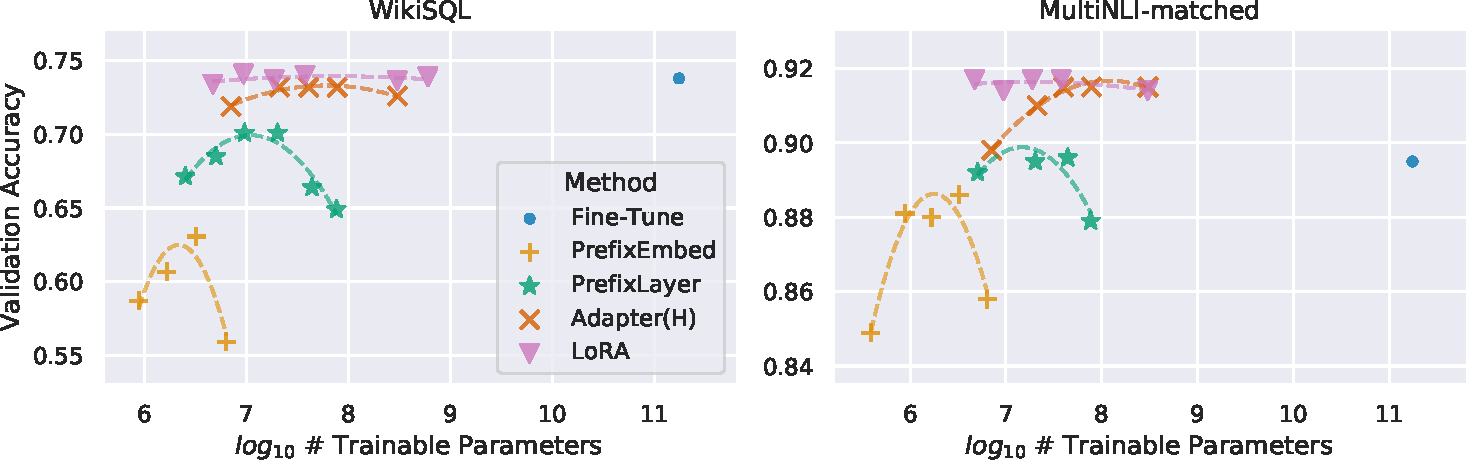
\includegraphics[width=0.97\textwidth]{figures/LoRA_wikisql.pdf}
\caption{GPT-3 175B validation accuracy vs. number of trainable parameters of several adaptation methods on WikiSQL and MNLI-matched. LoRA exhibits better scalability and task performance. See~\autoref{app:gpt3_extra} for more details on the plotted data points.}
\label{fig:eff}
\end{figure}

